\documentclass{beamer}
\usepackage{ragged2e}
\usepackage{CJKutf8}
\usepackage{tikz}
\setbeamertemplate{theorems}[numbered]

\begin{document}
\begin{CJK*}{UTF8}{gbsn}

\newtheorem{Thm}{定理}[section]
\theoremstyle{definition}
\newtheorem{Def}{定义}[section]
\theoremstyle{example}
\newtheorem*{Ex}{例:}
\date{}
\author{陈建文}

\title{第十章 有向图}
\begin{frame}
  \titlepage
\end{frame}  
\section{有向图的概念}
\begin{frame}
  \frametitle{1. 有向图的概念}

  \begin{Def}\justifying\let\raggedright\justifying
    设$V$为一个有穷非空集合,$A \subseteq V\times V \setminus \{(v,v)|v \in V\}$,二元组$D=(V,A)$称为一个\alert{有向图}。$V$称为有向图$D$的\alert{顶点集},$V$中的元素称为$D$的\alert{顶点}。
    $A$称为$D$的\alert{弧集}或\alert{有向边集},$A$中的元素称为$D$的\alert{弧}或\alert{有向边}。如果$x = (u,v) \in A$,则$u$称为弧$x$的\alert{起点},$v$称为弧$x$的\alert{终点}。
  \end{Def}
    \centering
  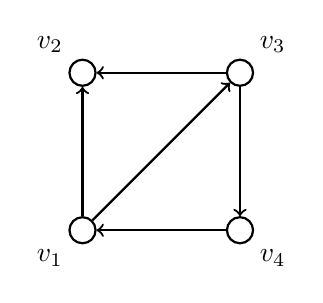
\begin{tikzpicture}[auto,
    specification/.style ={circle, draw, thick}]
   \node[specification] (A) [label=-135:$v_1$] at (0,0)  {};
   \node[specification] (B) [label=135:$v_2$] at (0,2)  {};
   \node[specification] (C) [label=45:$v_3$] at (2,2)  {};
   \node[specification] (D) [label=-45:$v_4$] at (2,0)  {};
   \draw[thick, ->] (A) to  (B);
   \draw[thick, ->] (C) to  (B);
   \draw[thick, ->] (C) to  (D);
   \draw[thick, ->] (D) to  (A);
   \draw[thick, ->] (A) to  (C);
\end{tikzpicture}

\end{frame}

\begin{frame}
  \frametitle{1. 有向图的概念}
  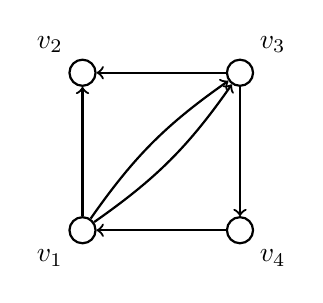
\begin{tikzpicture}[auto,
    specification/.style ={circle, draw, thick}]
   \node[specification] (A) [label=-135:$v_1$] at (0,0)  {};
   \node[specification] (B) [label=135:$v_2$] at (0,2)  {};
   \node[specification] (C) [label=45:$v_3$] at (2,2)  {};
   \node[specification] (D) [label=-45:$v_4$] at (2,0)  {};
   \draw[thick, ->] (A) to  (B);
   \draw[thick, ->] (C) to  (B);
   \draw[thick, ->] (C) to  (D);
   \draw[thick, ->] (D) to  (A);
   \draw[thick, ->] (A) to [bend left = 10] (C);
   \draw[thick, ->] (A) to [bend right = 10] (C);
\end{tikzpicture}\hspace{1cm}
  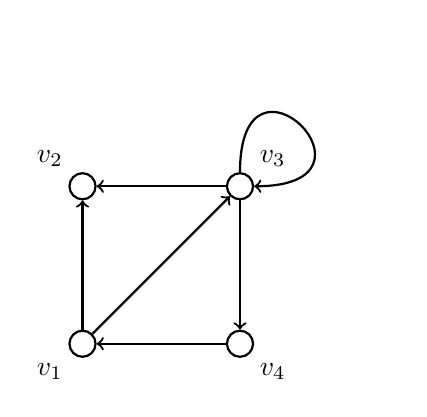
\begin{tikzpicture}[auto,
    specification/.style ={circle, draw, thick}]
   \node[specification] (A) [label=-135:$v_1$] at (0,0)  {};
   \node[specification] (B) [label=135:$v_2$] at (0,2)  {};
   \node[specification] (C) [label=45:$v_3$] at (2,2)  {};
   \node[specification] (D) [label=-45:$v_4$] at (2,0)  {};
   \draw[thick, ->] (A) to  (B);
   \draw[thick, ->] (C) to  (B);
   \draw[thick, ->] (C) to  (D);
   \draw[thick, ->] (D) to  (A);
   \draw[thick, ->] (A) to  (C);
   \draw[thick, ->] (C) .. controls +(up:20mm) and +(right:20mm) .. (C);
\end{tikzpicture}

\end{frame}

\begin{frame}
  \frametitle{1. 有向图的概念}
  \begin{Def}
    如果$(u,v)$和$(v,u)$都是有向图$D$的弧,则称$(u,v)$与$(v,u)$为$D$的\alert{对称弧}。如果$D$中不含对称弧,则称$D$是\alert{定向图}。
  \end{Def}
  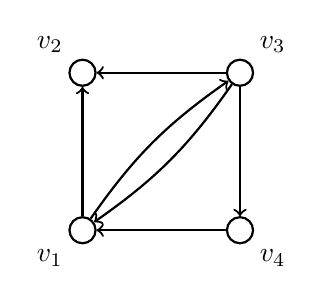
\begin{tikzpicture}[auto,
    specification/.style ={circle, draw, thick}]
   \node[specification] (A) [label=-135:$v_1$] at (0,0)  {};
   \node[specification] (B) [label=135:$v_2$] at (0,2)  {};
   \node[specification] (C) [label=45:$v_3$] at (2,2)  {};
   \node[specification] (D) [label=-45:$v_4$] at (2,0)  {};
   \draw[thick, ->] (A) to  (B);
   \draw[thick, ->] (C) to  (B);
   \draw[thick, ->] (C) to  (D);
   \draw[thick, ->] (D) to  (A);
   \draw[thick, ->] (A) to [bend left = 10] (C);
   \draw[thick, ->] (C) to [bend left = 10] (A);
\end{tikzpicture}\hspace{1cm}
  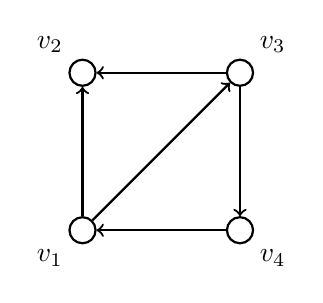
\begin{tikzpicture}[auto,
    specification/.style ={circle, draw, thick}]
   \node[specification] (A) [label=-135:$v_1$] at (0,0)  {};
   \node[specification] (B) [label=135:$v_2$] at (0,2)  {};
   \node[specification] (C) [label=45:$v_3$] at (2,2)  {};
   \node[specification] (D) [label=-45:$v_4$] at (2,0)  {};
   \draw[thick, ->] (A) to  (B);
   \draw[thick, ->] (C) to  (B);
   \draw[thick, ->] (C) to  (D);
   \draw[thick, ->] (D) to  (A);
   \draw[thick, ->] (A) to  (C);
\end{tikzpicture}
\end{frame}

\begin{frame}
  \frametitle{1. 有向图的概念}
  \begin{Def}
    设$D=(V,A)$是一个有向图,$D$的\alert{反向图}是有向图$D^T=(V,A^T)$,其中
    \[A^T=\{(u,v)|(v,u)\in A\}\]
  \end{Def}
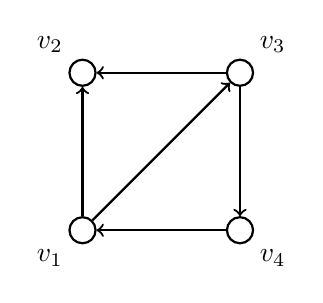
\begin{tikzpicture}[auto,
    specification/.style ={circle, draw, thick}]
   \node[specification] (A) [label=-135:$v_1$] at (0,0)  {};
   \node[specification] (B) [label=135:$v_2$] at (0,2)  {};
   \node[specification] (C) [label=45:$v_3$] at (2,2)  {};
   \node[specification] (D) [label=-45:$v_4$] at (2,0)  {};
   \draw[thick, ->] (A) to  (B);
   \draw[thick, ->] (C) to  (B);
   \draw[thick, ->] (C) to  (D);
   \draw[thick, ->] (D) to  (A);
   \draw[thick, ->] (A) to  (C);
\end{tikzpicture}\hspace{1cm}
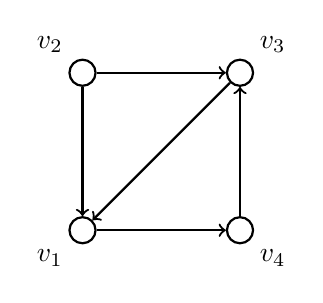
\begin{tikzpicture}[auto,
    specification/.style ={circle, draw, thick}]
   \node[specification] (A) [label=-135:$v_1$] at (0,0)  {};
   \node[specification] (B) [label=135:$v_2$] at (0,2)  {};
   \node[specification] (C) [label=45:$v_3$] at (2,2)  {};
   \node[specification] (D) [label=-45:$v_4$] at (2,0)  {};
   \draw[thick, ->] (B) to  (A);
   \draw[thick, ->] (B) to  (C);
   \draw[thick, ->] (D) to  (C);
   \draw[thick, ->] (A) to  (D);
   \draw[thick, ->] (C) to  (A);
\end{tikzpicture}
\end{frame}

\begin{frame}
  \frametitle{1. 有向图的概念}
  \begin{Def}
    设$D=(V,A)$是一个有向图,$v$是$D$的任一顶点,以$v$为终点的弧称为$v$的\alert{入弧};以$v$为始点的弧称为$v$的\alert{出弧}。顶点$v$的入弧的条数称为$v$的入度,记为$id(v)$;顶点$v$的出弧的条数称为$v$的\alert{出度},记为$od(v)$。
  \end{Def}
\centering
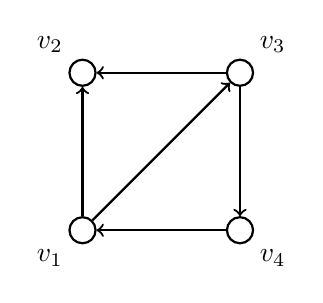
\begin{tikzpicture}[auto,
    specification/.style ={circle, draw, thick}]
   \node[specification] (A) [label=-135:$v_1$] at (0,0)  {};
   \node[specification] (B) [label=135:$v_2$] at (0,2)  {};
   \node[specification] (C) [label=45:$v_3$] at (2,2)  {};
   \node[specification] (D) [label=-45:$v_4$] at (2,0)  {};
   \draw[thick, ->] (A) to  (B);
   \draw[thick, ->] (C) to  (B);
   \draw[thick, ->] (C) to  (D);
   \draw[thick, ->] (D) to  (A);
   \draw[thick, ->] (A) to  (C);
\end{tikzpicture}  
\end{frame}

\begin{frame}
  \frametitle{1. 有向图的概念}
    \begin{Thm}
      设$D=(V,A)$是一个有向图,$|A| = q$,则
      \[\sum_{v\in V}id(v) = \sum_{v\in V}od(v) = q\]
      从而
      \[\sum_{v\in V}(id(v) + od(v)) = 2q\]
  \end{Thm}
\centering
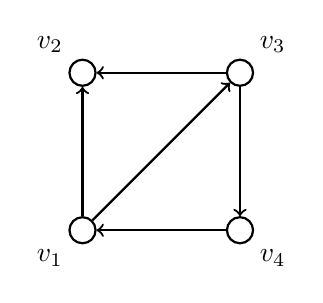
\begin{tikzpicture}[auto,
    specification/.style ={circle, draw, thick}]
   \node[specification] (A) [label=-135:$v_1$] at (0,0)  {};
   \node[specification] (B) [label=135:$v_2$] at (0,2)  {};
   \node[specification] (C) [label=45:$v_3$] at (2,2)  {};
   \node[specification] (D) [label=-45:$v_4$] at (2,0)  {};
   \draw[thick, ->] (A) to  (B);
   \draw[thick, ->] (C) to  (B);
   \draw[thick, ->] (C) to  (D);
   \draw[thick, ->] (D) to  (A);
   \draw[thick, ->] (A) to  (C);
\end{tikzpicture}  
\end{frame}

\begin{frame}
  \frametitle{1. 有向图的概念}
  \begin{Def}
     有向图$D=(V,A)$称为\alert{完全有向图},如果\[A=V\times V \setminus \{(v,v)| v \in V\}\]
   \end{Def}
   \centering
  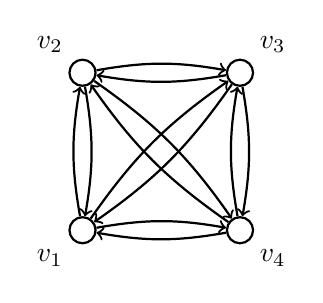
\begin{tikzpicture}[auto,
    specification/.style ={circle, draw, thick}]
   \node[specification] (A) [label=-135:$v_1$] at (0,0)  {};
   \node[specification] (B) [label=135:$v_2$] at (0,2)  {};
   \node[specification] (C) [label=45:$v_3$] at (2,2)  {};
   \node[specification] (D) [label=-45:$v_4$] at (2,0)  {};
   \draw[thick, ->] (A) to [bend left = 10]  (B);
   \draw[thick, ->] (B) to [bend left = 10]  (A);
   \draw[thick, ->] (B) to [bend left = 10]  (C);
   \draw[thick, ->] (C) to [bend left = 10]  (B);
   \draw[thick, ->] (C) to [bend left = 10]  (D);
   \draw[thick, ->] (D) to [bend left = 10]  (C);
   \draw[thick, ->] (D) to [bend left = 10]  (A);
   \draw[thick, ->] (A) to [bend left = 10]  (D);
   \draw[thick, ->] (B) to [bend left = 10]  (D);
   \draw[thick, ->] (D) to [bend left = 10]  (B);
   \draw[thick, ->] (A) to [bend left = 10]  (C);
   \draw[thick, ->] (C) to [bend left = 10]  (A);
\end{tikzpicture}   
\end{frame}

\begin{frame}
  \frametitle{1. 有向图的概念}
  \begin{Def}
    一个\alert{比赛图}为一个定向完全图,即任两个不同顶点间有且仅有一条弧。
  \end{Def}
  \centering
    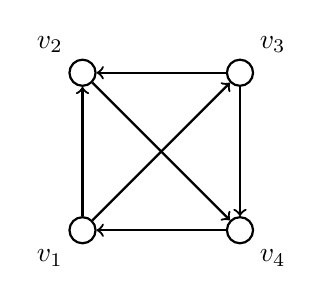
\begin{tikzpicture}[auto,
    specification/.style ={circle, draw, thick}]
   \node[specification] (A) [label=-135:$v_1$] at (0,0)  {};
   \node[specification] (B) [label=135:$v_2$] at (0,2)  {};
   \node[specification] (C) [label=45:$v_3$] at (2,2)  {};
   \node[specification] (D) [label=-45:$v_4$] at (2,0)  {};
   \draw[thick, ->] (A) to  (B);
   \draw[thick, ->] (C) to  (B);
   \draw[thick, ->] (C) to  (D);
   \draw[thick, ->] (D) to  (A);
   \draw[thick, ->] (A) to  (C);
   \draw[thick, ->] (B) to  (D);
 \end{tikzpicture}

\end{frame}

\begin{frame}
  \frametitle{1. 有向图的概念}
  \begin{Def}
    有向图$D=(V,A)$的\alert{补图}定义为$D^c=(V,A^c)$,其中
    \[A^c=(V \times V \setminus \{(v,v)|v \in V\})\setminus A\]
  \end{Def}
  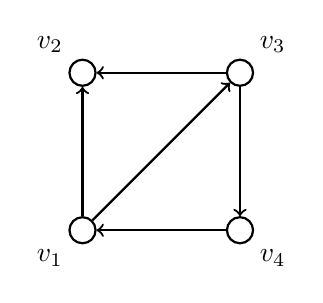
\begin{tikzpicture}[auto,
    specification/.style ={circle, draw, thick}]
   \node[specification] (A) [label=-135:$v_1$] at (0,0)  {};
   \node[specification] (B) [label=135:$v_2$] at (0,2)  {};
   \node[specification] (C) [label=45:$v_3$] at (2,2)  {};
   \node[specification] (D) [label=-45:$v_4$] at (2,0)  {};
   \draw[thick, ->] (A) to  (B);
   \draw[thick, ->] (C) to  (B);
   \draw[thick, ->] (C) to  (D);
   \draw[thick, ->] (D) to  (A);
   \draw[thick, ->] (A) to  (C);
 \end{tikzpicture}
\hspace{1cm}
 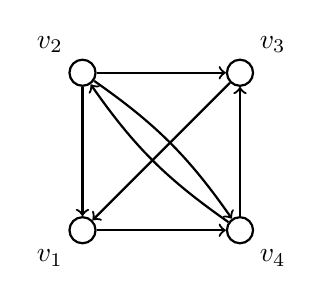
\begin{tikzpicture}[auto,
    specification/.style ={circle, draw, thick}]
   \node[specification] (A) [label=-135:$v_1$] at (0,0)  {};
   \node[specification] (B) [label=135:$v_2$] at (0,2)  {};
   \node[specification] (C) [label=45:$v_3$] at (2,2)  {};
   \node[specification] (D) [label=-45:$v_4$] at (2,0)  {};
   \draw[thick, ->] (B) to  (A);
   \draw[thick, ->] (B) to  (C);
   \draw[thick, ->] (D) to  (C);
   \draw[thick, ->] (A) to  (D);
   \draw[thick, ->] (C) to  (A);
   \draw[thick, ->] (B) to [bend left = 10]  (D);
   \draw[thick, ->] (D) to [bend left = 10]  (B);
\end{tikzpicture}

\end{frame}

\begin{frame}
  \frametitle{1. 有向图的概念}
  \begin{Def}\justifying\let\raggedright\justifying
    设$D_1=(V_1,A_1)$,$D_2=(V_2,A_2)$都为有向图,如果存在一个一一对应$\varphi:V_1 \to V_2$,使得$\forall u,v \in V_1, (u,v) \in A_1$当且仅当$(\varphi(u), \varphi(v)) \in A_2$,则称$D_1$与$D_2$\alert{同构}。
  \end{Def}
  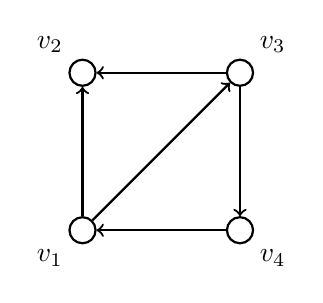
\begin{tikzpicture}[auto,
    specification/.style ={circle, draw, thick}]
   \node[specification] (A) [label=-135:$v_1$] at (0,0)  {};
   \node[specification] (B) [label=135:$v_2$] at (0,2)  {};
   \node[specification] (C) [label=45:$v_3$] at (2,2)  {};
   \node[specification] (D) [label=-45:$v_4$] at (2,0)  {};
   \draw[thick, ->] (A) to  (B);
   \draw[thick, ->] (C) to  (B);
   \draw[thick, ->] (C) to  (D);
   \draw[thick, ->] (D) to  (A);
   \draw[thick, ->] (A) to  (C);
 \end{tikzpicture}  \hspace{1cm}
   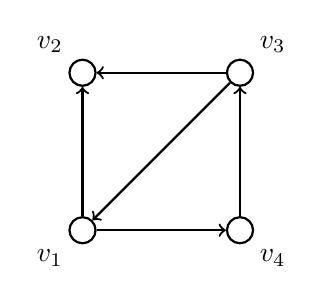
\begin{tikzpicture}[auto,
    specification/.style ={circle, draw, thick}]
   \node[specification] (A) [label=-135:$v_1$] at (0,0)  {};
   \node[specification] (B) [label=135:$v_2$] at (0,2)  {};
   \node[specification] (C) [label=45:$v_3$] at (2,2)  {};
   \node[specification] (D) [label=-45:$v_4$] at (2,0)  {};
   \draw[thick, ->] (A) to  (B);
   \draw[thick, ->] (C) to  (B);
   \draw[thick, ->] (D) to  (C);
   \draw[thick, ->] (C) to  (A);
   \draw[thick, ->] (A) to  (D);
\end{tikzpicture} 
\end{frame}

\begin{frame}
  \frametitle{1. 有向图的概念}
  \begin{Def}\justifying\let\raggedright\justifying
    设$D=(V,A)$为一个有向图,有向图$H=(V_1,A_1)$称为$D$的一个\alert{子图},如果
    $V_1$为$V$的非空子集,$A_1$为$A$的子集。
如果$H \neq D$,则称$H$为$D$的\alert{真子图}。
\end{Def}
  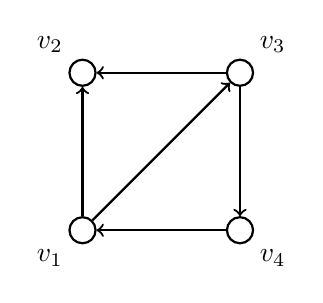
\begin{tikzpicture}[auto,
    specification/.style ={circle, draw, thick}]
   \node[specification] (A) [label=-135:$v_1$] at (0,0)  {};
   \node[specification] (B) [label=135:$v_2$] at (0,2)  {};
   \node[specification] (C) [label=45:$v_3$] at (2,2)  {};
   \node[specification] (D) [label=-45:$v_4$] at (2,0)  {};
   \draw[thick, ->] (A) to  (B);
   \draw[thick, ->] (C) to  (B);
   \draw[thick, ->] (C) to  (D);
   \draw[thick, ->] (D) to  (A);
   \draw[thick, ->] (A) to  (C);
 \end{tikzpicture}
\hspace{1cm}
   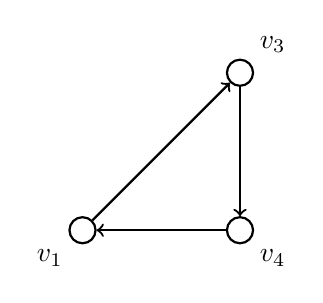
\begin{tikzpicture}[auto,
    specification/.style ={circle, draw, thick}]
   \node[specification] (A) [label=-135:$v_1$] at (0,0)  {};
%   \node[specification] (B) [label=135:$v_2$] at (0,2)  {};
   \node[specification] (C) [label=45:$v_3$] at (2,2)  {};
   \node[specification] (D) [label=-45:$v_4$] at (2,0)  {};
%   \draw[thick, ->] (A) to  (B);
 %  \draw[thick, ->] (C) to  (B);
   \draw[thick, ->] (C) to  (D);
   \draw[thick, ->] (D) to  (A);
   \draw[thick, ->] (A) to  (C);
 \end{tikzpicture}

\end{frame}
\begin{frame}
  \frametitle{1. 有向图的概念}
  \begin{Def}
        设$D=(V,A)$为一个有向图,如果$F\subseteq A$,则称$D$的子图$H=(V,F)$ 为$D$的一个\alert{生成子图}。
\end{Def}
  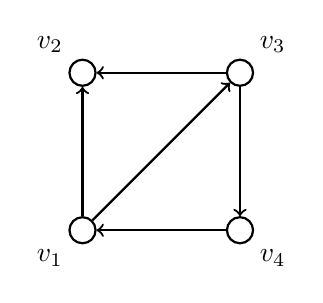
\begin{tikzpicture}[auto,
    specification/.style ={circle, draw, thick}]
   \node[specification] (A) [label=-135:$v_1$] at (0,0)  {};
   \node[specification] (B) [label=135:$v_2$] at (0,2)  {};
   \node[specification] (C) [label=45:$v_3$] at (2,2)  {};
   \node[specification] (D) [label=-45:$v_4$] at (2,0)  {};
   \draw[thick, ->] (A) to  (B);
   \draw[thick, ->] (C) to  (B);
   \draw[thick, ->] (C) to  (D);
   \draw[thick, ->] (D) to  (A);
   \draw[thick, ->] (A) to  (C);
 \end{tikzpicture}\hspace{1cm}
   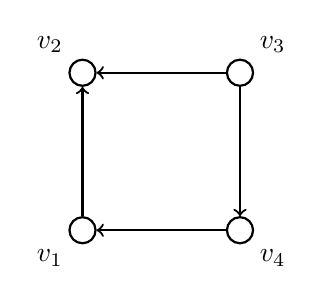
\begin{tikzpicture}[auto,
    specification/.style ={circle, draw, thick}]
   \node[specification] (A) [label=-135:$v_1$] at (0,0)  {};
   \node[specification] (B) [label=135:$v_2$] at (0,2)  {};
   \node[specification] (C) [label=45:$v_3$] at (2,2)  {};
   \node[specification] (D) [label=-45:$v_4$] at (2,0)  {};
   \draw[thick, ->] (A) to  (B);
   \draw[thick, ->] (C) to  (B);
   \draw[thick, ->] (C) to  (D);
   \draw[thick, ->] (D) to  (A);
 \end{tikzpicture}
\end{frame}

\begin{frame}
  \frametitle{1. 有向图的概念}
  \begin{Def}
    设$D=(V,A)$为一个有向图,如果$S \subseteq V$,则$S$的\alert{导出子图}定义为$H=(S,F)$,其中
    \[F=\{(u,v)\in A | u \in S, v \in S\}\]
\end{Def}
  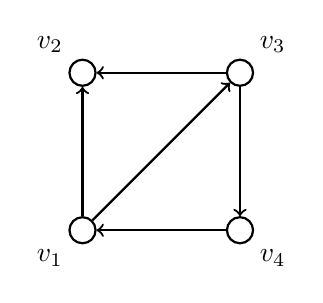
\begin{tikzpicture}[auto,
    specification/.style ={circle, draw, thick}]
   \node[specification] (A) [label=-135:$v_1$] at (0,0)  {};
   \node[specification] (B) [label=135:$v_2$] at (0,2)  {};
   \node[specification] (C) [label=45:$v_3$] at (2,2)  {};
   \node[specification] (D) [label=-45:$v_4$] at (2,0)  {};
   \draw[thick, ->] (A) to  (B);
   \draw[thick, ->] (C) to  (B);
   \draw[thick, ->] (C) to  (D);
   \draw[thick, ->] (D) to  (A);
   \draw[thick, ->] (A) to  (C);
 \end{tikzpicture}
 \hspace{1cm}
  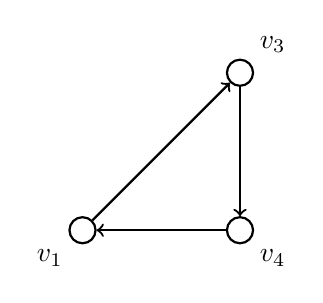
\begin{tikzpicture}[auto,
    specification/.style ={circle, draw, thick}]
   \node[specification] (A) [label=-135:$v_1$] at (0,0)  {};
%   \node[specification] (B) [label=135:$v_2$] at (0,2)  {};
   \node[specification] (C) [label=45:$v_3$] at (2,2)  {};
   \node[specification] (D) [label=-45:$v_4$] at (2,0)  {};
%   \draw[thick, ->] (A) to  (B);
%   \draw[thick, ->] (C) to  (B);
   \draw[thick, ->] (C) to  (D);
   \draw[thick, ->] (D) to  (A);
   \draw[thick, ->] (A) to  (C);
 \end{tikzpicture} 
\end{frame}

\section{2. 有向路和有向圈}
\begin{frame}
  \frametitle{2. 有向路和有向圈}
  \begin{Def}
    设$D=(V,A)$为一个有向图。$D$的顶点和弧的交错序列
    \[v_0,x_1,v_1,x_2,v_2,\cdots,v_{n-1},x_n,v_n \]
    称为$D$的一个\alert{有向通道},如果$x_i = (v_{i-1},v_i)$, $i=1,2,\cdots, n$。 \\$n$称为该有向通道的长。 如果$v_0=v_n$,则称它是\alert{闭有向通道}。
  \end{Def}
  \centering
  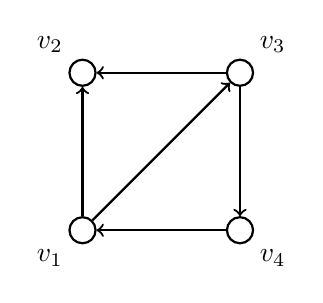
\begin{tikzpicture}[auto,
    specification/.style ={circle, draw, thick}]
   \node[specification] (A) [label=-135:$v_1$] at (0,0)  {};
   \node[specification] (B) [label=135:$v_2$] at (0,2)  {};
   \node[specification] (C) [label=45:$v_3$] at (2,2)  {};
   \node[specification] (D) [label=-45:$v_4$] at (2,0)  {};
   \draw[thick, ->] (A) to  (B);
   \draw[thick, ->] (C) to  (B);
   \draw[thick, ->] (C) to  (D);
   \draw[thick, ->] (D) to  (A);
   \draw[thick, ->] (A) to  (C);
 \end{tikzpicture}      
\end{frame}

\begin{frame}
  \frametitle{2. 有向路和有向圈}
  \begin{Def}
设$D=(V,A)$为一个有向图,$D$的一条\alert{有向迹}是$D$的一条所有弧均不相同的有向通道。起点和终点相同的迹称为\alert{闭迹}。迹上出现的弧的条数称为迹的长。   
  \end{Def}
  \centering
  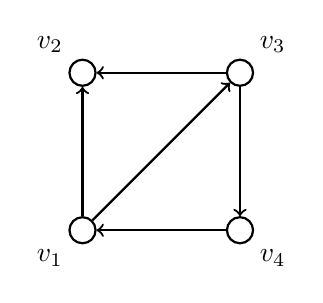
\begin{tikzpicture}[auto,
    specification/.style ={circle, draw, thick}]
   \node[specification] (A) [label=-135:$v_1$] at (0,0)  {};
   \node[specification] (B) [label=135:$v_2$] at (0,2)  {};
   \node[specification] (C) [label=45:$v_3$] at (2,2)  {};
   \node[specification] (D) [label=-45:$v_4$] at (2,0)  {};
   \draw[thick, ->] (A) to  (B);
   \draw[thick, ->] (C) to  (B);
   \draw[thick, ->] (C) to  (D);
   \draw[thick, ->] (D) to  (A);
   \draw[thick, ->] (A) to  (C);
 \end{tikzpicture}      
\end{frame}

\begin{frame}
  \frametitle{2. 有向路和有向圈}
  \begin{Def}
设$D=(V,A)$为一个有向图,$D$的一条不含重复顶点的有向通道称为$D$的一条\alert{有向路}。有向路上弧的条数称为该有向路的长。一条至少含有两个不同顶点的闭有向通道称为一个\alert{有向圈},如果该闭有向通道上除起点和终点外各顶点互不相同。
  \end{Def}
  \centering
  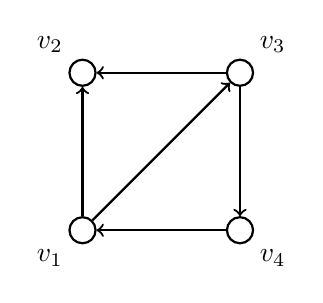
\begin{tikzpicture}[auto,
    specification/.style ={circle, draw, thick}]
   \node[specification] (A) [label=-135:$v_1$] at (0,0)  {};
   \node[specification] (B) [label=135:$v_2$] at (0,2)  {};
   \node[specification] (C) [label=45:$v_3$] at (2,2)  {};
   \node[specification] (D) [label=-45:$v_4$] at (2,0)  {};
   \draw[thick, ->] (A) to  (B);
   \draw[thick, ->] (C) to  (B);
   \draw[thick, ->] (C) to  (D);
   \draw[thick, ->] (D) to  (A);
   \draw[thick, ->] (A) to  (C);
 \end{tikzpicture}      
\end{frame}
\begin{frame}
  \frametitle{2. 有向路和有向圈}
  \begin{Def}
含有向图$D$的所有顶点的有向圈称为$D$的\alert{生成有向圈},或\alert{有向哈密顿圈}。
有生成有向圈的有向图称
为\alert{有向哈密顿图}。含有向图$D$的所有顶点的有向路称为$D$的\alert{生成有向路},
或\alert{有向哈密顿路}。
  \end{Def}
  \centering
  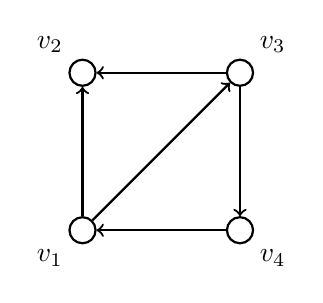
\begin{tikzpicture}[auto,
    specification/.style ={circle, draw, thick}]
   \node[specification] (A) [label=-135:$v_1$] at (0,0)  {};
   \node[specification] (B) [label=135:$v_2$] at (0,2)  {};
   \node[specification] (C) [label=45:$v_3$] at (2,2)  {};
   \node[specification] (D) [label=-45:$v_4$] at (2,0)  {};
   \draw[thick, ->] (A) to  (B);
   \draw[thick, ->] (C) to  (B);
   \draw[thick, ->] (C) to  (D);
   \draw[thick, ->] (D) to  (A);
   \draw[thick, ->] (A) to  (C);
 \end{tikzpicture}      
\end{frame}

\begin{frame}
  \frametitle{2. 有向路和有向圈}
  \begin{Def}
    设$D=(V,A)$是一个有向图,$u$和$v$是$D$的顶点。如果在$D$中有一条从$u$到$v$的
    有向路,则称从$u$能达到$v$,或者$v$是从$u$\alert{可达}的。
  \end{Def}
  \centering
  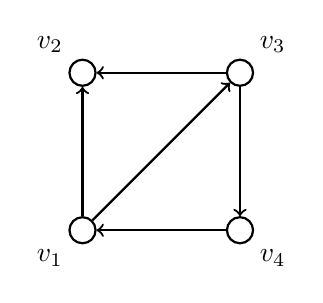
\begin{tikzpicture}[auto,
    specification/.style ={circle, draw, thick}]
   \node[specification] (A) [label=-135:$v_1$] at (0,0)  {};
   \node[specification] (B) [label=135:$v_2$] at (0,2)  {};
   \node[specification] (C) [label=45:$v_3$] at (2,2)  {};
   \node[specification] (D) [label=-45:$v_4$] at (2,0)  {};
   \draw[thick, ->] (A) to  (B);
   \draw[thick, ->] (C) to  (B);
   \draw[thick, ->] (C) to  (D);
   \draw[thick, ->] (D) to  (A);
   \draw[thick, ->] (A) to  (C);
 \end{tikzpicture}      
\end{frame}

\begin{frame}
  \frametitle{2. 有向路和有向圈}
  \begin{Def}
   有向图$D$称为是\alert{强连通}的,如果对$D$的任两个不同的顶点$u$和$v$,$u$和$v$是互达的。 
  \end{Def}
  \centering
  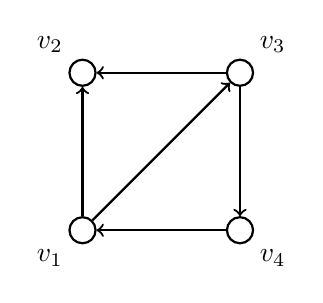
\begin{tikzpicture}[auto,
    specification/.style ={circle, draw, thick}]
   \node[specification] (A) [label=-135:$v_1$] at (0,0)  {};
   \node[specification] (B) [label=135:$v_2$] at (0,2)  {};
   \node[specification] (C) [label=45:$v_3$] at (2,2)  {};
   \node[specification] (D) [label=-45:$v_4$] at (2,0)  {};
   \draw[thick, ->] (A) to  (B);
   \draw[thick, ->] (C) to  (B);
   \draw[thick, ->] (C) to  (D);
   \draw[thick, ->] (D) to  (A);
   \draw[thick, ->] (A) to  (C);
 \end{tikzpicture}      
\end{frame}

\begin{frame}
  \frametitle{2. 有向路和有向圈}
  \begin{Def}
   有向图$D$的极大强连通子图称为$D$的一个\alert{强支}。 
  \end{Def}
  \centering
  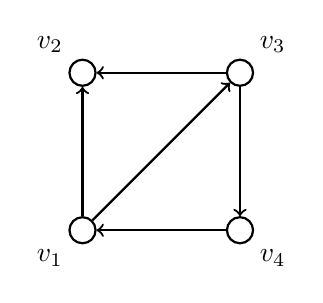
\begin{tikzpicture}[auto,
    specification/.style ={circle, draw, thick}]
   \node[specification] (A) [label=-135:$v_1$] at (0,0)  {};
   \node[specification] (B) [label=135:$v_2$] at (0,2)  {};
   \node[specification] (C) [label=45:$v_3$] at (2,2)  {};
   \node[specification] (D) [label=-45:$v_4$] at (2,0)  {};
   \draw[thick, ->] (A) to  (B);
   \draw[thick, ->] (C) to  (B);
   \draw[thick, ->] (C) to  (D);
   \draw[thick, ->] (D) to  (A);
   \draw[thick, ->] (A) to  (C);
 \end{tikzpicture}      
\end{frame}

\begin{frame}
  \frametitle{2. 有向路和有向圈}
    \begin{Thm}
    设$D=(V,A)$是一个有向图。在$V$上定义二元关系$\cong$如下:\[\forall u, v \in V, u \cong v\text{当且仅当}u\text{与}v\text{互达}\]则$\cong$是$V$上的等价关系,$D$的强支就是关于$\cong$的每个等价类的导出子图。
  \end{Thm}
  \centering
  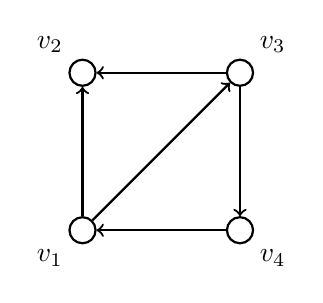
\begin{tikzpicture}[auto,
    specification/.style ={circle, draw, thick}]
   \node[specification] (A) [label=-135:$v_1$] at (0,0)  {};
   \node[specification] (B) [label=135:$v_2$] at (0,2)  {};
   \node[specification] (C) [label=45:$v_3$] at (2,2)  {};
   \node[specification] (D) [label=-45:$v_4$] at (2,0)  {};
   \draw[thick, ->] (A) to  (B);
   \draw[thick, ->] (C) to  (B);
   \draw[thick, ->] (C) to  (D);
   \draw[thick, ->] (D) to  (A);
   \draw[thick, ->] (A) to  (C);
 \end{tikzpicture}      
\end{frame}

\begin{frame}
  \frametitle{2. 有向路和有向圈}
  \begin{Def}
   有向图$D=(V,A)$称为\alert{单向连通}的,如果对$D$的任两个不同顶点$u$和$v$,或从$u$可达到$v$,或从$v$可达到$u$。 
  \end{Def}
  \centering
  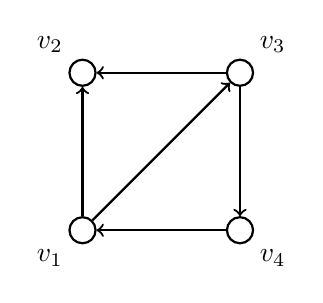
\begin{tikzpicture}[auto,
    specification/.style ={circle, draw, thick}]
   \node[specification] (A) [label=-135:$v_1$] at (0,0)  {};
   \node[specification] (B) [label=135:$v_2$] at (0,2)  {};
   \node[specification] (C) [label=45:$v_3$] at (2,2)  {};
   \node[specification] (D) [label=-45:$v_4$] at (2,0)  {};
   \draw[thick, ->] (A) to  (B);
   \draw[thick, ->] (C) to  (B);
   \draw[thick, ->] (C) to  (D);
   \draw[thick, ->] (D) to  (A);
   \draw[thick, ->] (A) to  (C);
 \end{tikzpicture}      
\end{frame}

\begin{frame}
  \frametitle{2. 有向路和有向圈}
  \begin{Def}
   有向图$D=(V,A)$为一个有向图,如果抹去$D$中所有弧的方向之后所得到的无向图是连通的,则称$D$为\alert{弱连通}的,简称\alert{连通}的。 
  \end{Def}
  \centering
  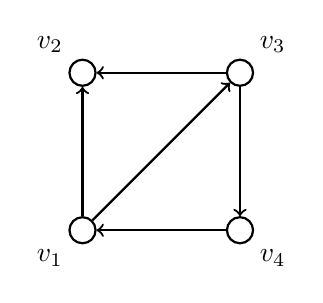
\begin{tikzpicture}[auto,
    specification/.style ={circle, draw, thick}]
   \node[specification] (A) [label=-135:$v_1$] at (0,0)  {};
   \node[specification] (B) [label=135:$v_2$] at (0,2)  {};
   \node[specification] (C) [label=45:$v_3$] at (2,2)  {};
   \node[specification] (D) [label=-45:$v_4$] at (2,0)  {};
   \draw[thick, ->] (A) to  (B);
   \draw[thick, ->] (C) to  (B);
   \draw[thick, ->] (C) to  (D);
   \draw[thick, ->] (D) to  (A);
   \draw[thick, ->] (A) to  (C);
 \end{tikzpicture}      
\end{frame}


\section{3. 强连通图的应用}
\section{4. 有向图的邻接矩阵}
\begin{frame}
  \frametitle{4. 有向图的邻接矩阵}
  \centering
  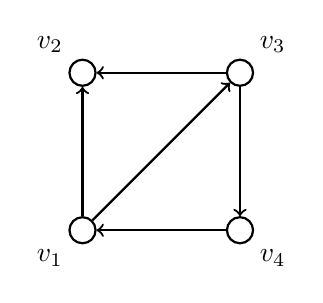
\begin{tikzpicture}[auto,
    specification/.style ={circle, draw, thick}]
   \node[specification] (A) [label=-135:$v_1$] at (0,0)  {};
   \node[specification] (B) [label=135:$v_2$] at (0,2)  {};
   \node[specification] (C) [label=45:$v_3$] at (2,2)  {};
   \node[specification] (D) [label=-45:$v_4$] at (2,0)  {};
   \draw[thick, ->] (A) to  (B);
   \draw[thick, ->] (C) to  (B);
   \draw[thick, ->] (C) to  (D);
   \draw[thick, ->] (D) to  (A);
   \draw[thick, ->] (A) to  (C);
 \end{tikzpicture}    
\end{frame}

\begin{frame}
  \frametitle{4. 有向图的邻接矩阵}
  \begin{Thm}
   设$B$是有向图$D=(V,A)$的邻接矩阵,$V=\{v_1,v_2,\cdots,v_p\}$,则从顶点$v_i$到顶点$v_j$的长为$l$的有向通道的条数等于$B^l$的第$i$行第$j$列元素$(B^l)_{ij}$的值。 
  \end{Thm}
\end{frame}

\begin{frame}
  \frametitle{4. 有向图的邻接矩阵}
  \begin{Thm}
    设$p \times p$矩阵$B$是有向图$D=(V,A)$的邻接矩阵,则$D$的可达矩阵
    \[R = I \lor B \lor B^{(2)} \lor \cdots \lor B^{(p-1)}\]
  \end{Thm}
\end{frame}

\begin{frame}
  \frametitle{4. 有向图的邻接矩阵}
  \begin{Thm}
   设$p \times p$矩阵$R$为有向图$D=(V,A)$的可达矩阵, \[C=R \land R^T,\] $C$的第$i$行上为$1$的元素$c_{ij_1}, c_{ij_2}, \ldots, c_{ij_k}$,则$v_i$在由$V_i= \{v_{j_1}, v_{j_2}, \ldots, v_{j_k}\}$诱导出的$D$的子图-$D$的强支中。
 \end{Thm}
  \centering
  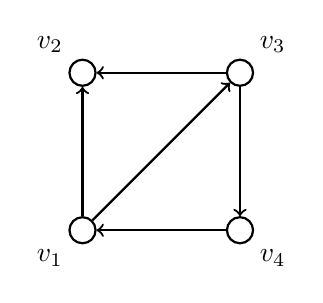
\begin{tikzpicture}[auto,
    specification/.style ={circle, draw, thick}]
   \node[specification] (A) [label=-135:$v_1$] at (0,0)  {};
   \node[specification] (B) [label=135:$v_2$] at (0,2)  {};
   \node[specification] (C) [label=45:$v_3$] at (2,2)  {};
   \node[specification] (D) [label=-45:$v_4$] at (2,0)  {};
   \draw[thick, ->] (A) to  (B);
   \draw[thick, ->] (C) to  (B);
   \draw[thick, ->] (C) to  (D);
   \draw[thick, ->] (D) to  (A);
   \draw[thick, ->] (A) to  (C);
 \end{tikzpicture}     
\end{frame}
\section{5. 有向树与有序树}
\begin{frame}
  \frametitle{5. 有向树与有序树}
  \begin{Def}
    一个有向图,如果抹去其所有弧的方向以后所得到的无向图是一棵无向树,则称该有向图为一棵\alert{有向树}。
  \end{Def}
\end{frame}
\begin{frame}
  \frametitle{5. 有向树与有序树}
  \begin{Def}
    有向树$D$称为\alert{有根树},如果$D$中恰有一个顶点的入度为0,而其余每个顶点的入度均为1。有根树中入度为0的顶点称为有根树的根,出度为0的顶点称为\alert{叶子},非叶顶点称为\alert{分支点}或\alert{内顶点}。
  \end{Def}
\end{frame}

\begin{frame}
  \frametitle{5. 有向树与有序树}
  \begin{Def}
  设$T=(V,A)$为一棵有根树。如果$(u,v)\in A$,则称$v$为$u$的\alert{儿子},$u$为$v$的\alert{父亲}。如果从顶点$u$能达到顶点$v$,则称$v$为$u$的\alert{子孙},$u$为$v$的\alert{祖先}。如果$u$是$v$的祖先且$u \neq v$,则称$u$为$v$的\alert{真祖先},$v$为$u$的\alert{真子孙}。
  \end{Def}
\end{frame}

\begin{frame}
  \frametitle{5. 有向树与有序树}
  \begin{Def}\justifying\let\raggedright\justifying
    设$T=(V,A)$为一棵以$v_0$为根的有根树。从$v_0$到顶点$v$的有向路的长度称为$T$的顶点$v$的\alert{深度}。从顶点$v$到$T$的叶子的最长的有向路的长度称为顶点$v$在$T$中的\alert{高度}。根顶点$v_0$的高度称为树$T$的\alert{高度}。
  \end{Def}
\end{frame}

\begin{frame}
  \frametitle{5. 有向树与有序树}
  \begin{Def}
    设$T=(V,A)$为一棵有根树,$v$是$T$的一个顶点,由$v$及其子孙所导出的$T$的子图称为$T$的以$v$为根的\alert{子树}。
  \end{Def}
\end{frame}

\begin{frame}
  \frametitle{5. 有向树与有序树}
  \begin{Def}
    设$T=(V,A)$为一棵有根树。如果$T$的每个顶点的各个儿子排定了次序,则称$T$为一
    棵\alert{有序树}。
  \end{Def}
\end{frame}

\begin{frame}
  \frametitle{5. 有向树与有序树}
  \begin{Def}
    有序树$T$称为\alert{$m$元有序树},如果$T$的每个顶点的出度$\leq m$。一棵$m$元
    有序树$T$称为\alert{正则$m$元有序树},如果$T$的每个顶点的出度不是$0$就是$m$。
    二元有序树简称\alert{二元树}。
  \end{Def}
\end{frame}

%%% Local Variables:
%%% mode: latex
%%% TeX-master: "chapter10"
%%% End:

\end{CJK*}
\end{document}

%%% Local Variables:
%%% mode: latex
%%% TeX-master: t
%%% End:
